\documentclass[aps, prc, reprint, amsmath, groupedaddress, nofootinbib]{revtex4-1}
%\usepackage[compat=1.1.0]{tikz-feynman}
\usepackage[utf8]{inputenc}
\usepackage{hyperref}
\usepackage{amsmath}
\usepackage{amssymb}
\usepackage{amsfonts}
\usepackage{tabularx}
\usepackage{booktabs}
\usepackage{graphicx}
\usepackage{color}
\usepackage{multirow}
\usepackage{verbatim}
\usepackage[inline]{enumitem}
\graphicspath{{fig/}}
\definecolor{theblue}{RGB}{0,50,230}
\usepackage{appendix}
\hypersetup{
  colorlinks=true,
  linkcolor=theblue,
  citecolor=theblue,
  urlcolor=theblue
} 
\usepackage[most]{tcolorbox}

\begin{abstract}
Energetic partons created in perturbative processes at the onset of relativistic heavy-ion collisions are excellent probes for the study of hot and dense deconfined QCD matter.
Transport approaches, that allow for the realistic description of fluctuating initial conditions and medium properties, have become a powerful tool in this endeavor. 
However, the implementation of the Landau-Pomeranchuk-Migdal (LPM) effect for medium induced splitting processes, poses a challenge to a class of widely used models: the Boltzmann type transport equations.  
In this work, we investigated a possible solution, termed the ``modified Boltzmann transport" approach, including a prescription for the running coupling effect.
Fixing two parameters, outcomes of this approach are shown to agree with the splitting rates predicted by the next-to-lead-log solution of the AMY equation that works in the infinite medium limit and in the deep-LPM regime.
We also analyzed the behavior of this approach in a finite medium and an expanding medium, and found that future improvements are needed for this approach to work beyond the deep-LPM region.
This work will benefit transport model based studies and the usage of these models in the phenomenological extraction of the jet transport coefficient.


\end{abstract}

\begin{document}
\title{Monte-Carlo Modeling of the Landau-Pomeranchuk-Migdal effect for Medium-induced QCD Splitting Processes in the deep LPM regime}
\author{Weiyao Ke}
\author{Yingru Xu}
\author{Steffen A.\ Bass}
\affiliation{Department of Physics, Duke University, Durham, NC 27708-0305}
\date{\today}
\maketitle 

\section{Introduction}
The study of hard probes in relativistic heavy-ion collisions is moving towards the precision era thanks to upcoming experimental upgrades \cite{ATLAS-Collaboration:2012iwa,Abelevetal:2014dna,STAR:upgrade-hf,Adare:2015kwa,CMS:2017dec} as well as theoretical and computational advances that allow for the execution of jet propagations in a realistic Quark-Gluon-Plasma (QGP) medium (including event-by-event fluctuating initial conditions and temperature-dependent transport coefficients) \cite{Wang:1994fx,Zakharov:1996fv,Baier:1996sk,Zakharov:1997uu,Arnold:2002zm,Gyulassy:2003mc,Kovner:2003zj,CasalderreySolana:2007pr,Djordjevic:2008iz,Bass:2008rv,Schenke:2009gb,Majumder:2009zu,Majumder:2010qh,Armesto:2011ht,Zapp:2011ya,Ovanesyan:2011xy,Kang:2014xsa,Cao:2016gvr,Kauder:2018cdt,Cao:2017zih}. Among the goals for this research is the characterization of the QGP medium in terms of its jet transport coefficients $\hat{q}$.

Transport models are powerful tools that allow for the realistic description of fluctuating initial conditions and medium properties. 
However, the numerical implementation of the QCD analog of the Landau-Pomeranchuk-Migdal (LPM) effect, poses a serious challenge to a class of widely used models: the Boltzmann transport equations. 
In a dense medium, the LPM effect is important for the treatment medium-induced parton splitting processes where multiple scatterings act coherently \cite{PhysRev.103.1811,Wang:1994fx,Zakharov:1996fv,Zakharov:1997uu,Baier:1996kr,Baier:1996sk}.
Therefore, a medium-induced splitting becomes effectively an $n$-body to $(n+1)$-body process that extends in space-time.
This feature is particularly difficult to accurately accounted for in a Boltzmann transport equation, where interactions are usually based on few-body processes that are local.
To simplify the problem while still retaining essential qualitative features, different methods have been used in numerical studies \cite{Cao:2013ita,ColemanSmith:2012vr,Xu:2004mz,Zapp:2011ya,Gossiaux:2012cv,Park:thesis}.

In this work we try to identify what approximation we need to make in order to include the LPM effect in a Boltzmann-like transport model, the resultant technique is termed as ``the modified Boltzmann transport" approach. 
This approach can be tuned to semi-analytic calculations in an infinite medium limit in the deep LPM regime $xE \gg T$, and is also compared to other theoretical calculations performed in idealized limits 
 radiative processes to perturbative kinetic theory predictions in idealized limits \cite{Arnold:2002zm,Arnold:2008zu,Arnold:2009mr,Baier:1996kr,Baier:1998yf}. 
It reasonably describes the medium induced splitting rate for different channels $q\rightarrow q+g$, $g\rightarrow g+g$ and $g\rightarrow q+\bar{q}$, for a wide range of parton energies and at different coupling strengths.
A tentaive prescription for implementing running coupling is proposed and the results agrees quantitatively with theory expectations.
Therefore, the performance of this approach has been benchmarked in the deep LPM region to theoretical calculations. 
This practice is important for the future application of this transport model to a phenomenological extraction of the jet transport properties from systematic model-to-data comparison.

This paper is organized as follows. Section \ref{section:Boltzmann} introduces the Linearized Boltzmann plus Langevin transport model using incoherent calculation of parton splitting.
In Section \ref{section:modified-Boltzmann}, we propose an ansatz to modify the aforementioned model in Section \ref{section:Boltzmann} to include the LPM effect.
A next-to-leading-log (NLL) solution in the deep LPM region is used as guidance to determine the form of the ansatz.
Detailed comparisons between the simulation and the NLL solution is found in section \ref{section:results} and appendix \ref{app:tune-spectrum}.
The behavior of this approach in finite and expanding media is investigated in \ref{section:more}.
Finally, \ref{section:summary} is a short summary and outlook.



\section{Transport approach in the incoherent limit}\label{section:Boltzmann}
In this section, we describe the Monte Carlo model in detail. The partonic processes are categorized into elastic (particle number conserving) and inelastic processes (particle number non-conserving). 
The inelastic processes are further divided into parton-splitting and parton-jointing contribution. 
In this section, we shall first proceed using local and incoherent calculation of such processes and will discuss in great detail in the next section on including the LPM effect in a Boltzmann-like transport approach.

The elastic interaction between hard parton and medium is separate into a large-momentum transfer (hard) and a small-momentum transfer (soft) part.
The switching scale is chosen to be proportional to the Debye mass square $Q_{\textrm{cut}}^2 = c m_D^2$, where $c$ is a parameter.
Respectively, the inelastic processes are also separated into diffusion-induced slitting / jointing processes, and large-$Q$ matrix-element based inelastic scattering contribution.

The large-$Q$ collisions are solved by a linearized Boltzmann equation with using collision rates calculated with vacuum matrix-elements, while the soft interactions are approximated by a diffusion process and is solved by Langevin equations.
This combined Langevin and linearized Boltzmann dyanmics is solved on the particle level using a two step approach,
\begin{eqnarray}
\vec{x}(t+\Delta t) &=& \frac{\vec{p}}{E}\Delta t\\
\vec{p}_{\textrm{int}} &=& \vec{p} - \eta_D \vec{p} \Delta t + \vec{\xi}(t) \Delta t\\
\Delta t\frac{dR(T, \vec{v}, \vec{p}_{\textrm{int}})}{d\vec{p}^3} &\xrightarrow{\textrm{sampling}}& \vec{p}(t+\Delta t)
\end{eqnarray}
Where the particle first does free transport, and then its momentum be updated with diffusion dynamics to get an intermediate $\vec{p}_{\textrm{int}}$. 
Then, the particle under goes collision according to the reaction probability within $\Delta t$, and the final states are obtained by sampling the differential collision rate.
The diffusion dynamics consists of a thermal random force such that,
\begin{eqnarray}
\left\langle\xi_i(t)\xi_j(0)\right\rangle = \delta(t) \left(
\frac{p_i p_j}{p^2}\hat{q}_{S, L} + \left(
\delta_{ij}-\frac{p_i p_j}{p^2}
\right)\frac{\hat{q}_S}{2} 
\right)
\end{eqnarray}
Because we require that the diffusion dynamics only accounts for soft momentum transfer processes, its transport coefficient is obtained by integrating the leading order collision kernel upto the momentum $Q_{\textrm{cut}}$,
\begin{eqnarray}
\hat{q}_S = \int dq^2 \frac{\alpha_s m_D^2 T}{q^2 (q^2+m_D^2)} \\
\hat{q}_{S,L} = \int dq^2 \frac{\alpha_s m_\infty^2 T}{q^2 (q^2+m_\infty^2)}
\end{eqnarray}
with the drag coefficient determined by the Einstein relation,
\begin{eqnarray}
\eta_D = \frac{\hat{q}_{S,L}}{2ET} - \frac{d\hat{q}_{S,L}}{dp^2} - \frac{2\hat{q}_{S,L} - 2\hat{q}_S}{2p^2}
\end{eqnarray}
For the large-$Q$ scattering processes, the collision rates for the $2\rightarrow 2$ and $2\rightarrow 3$ scatterings are obtained by integrating the vacuum matrix-element,
\begin{eqnarray}
R = \frac{d}{2E_1}\int  \frac{d^3p_2}{2E_2(2\pi)^3} f_0(p_2)2\hat{s} \int_{-\hat{s}}^{Q_{\textrm{cut}^2}}\frac{d\sigma}{d\hat{t}}d\hat{t}
\end{eqnarray}
The integration is restricted to large momentum transfer above $Q_{\textrm{cut}}$ and therefore we do not impose additional screening effect to regulate the matrix-element.
For the incoherent diffusion-induced splitting rate, we borrow the expression from [] stripping its time-dependent phase factor,
\begin{eqnarray}
R = \int d k_\perp^2 dx \frac{\alpha_s P(x) \hat{q}^S}{2\pi (k_\perp^2 + m_\infty^2)^2}
\end{eqnarray}
where a gluon thermal mass is added to screen the divergence.
For the reverse processes $3\rightarrow 2$  and $2\rightarrow 1$ processes, similar reaction rate can be written down.

The vacuum matrix-element is used for the large-$Q$ elastic and inelastic scatterings.
In this work, the $2\rightarrow 2$ matrix-element only includes the $\hat{t}$-channel contribution.
Regarding the $2\rightarrow 3$ matrix-element, in previous study [], we used to employ an improved version of the original Gunion-Bertsch cross-section that works under the limits $k_\perp, q_\perp \ll \sqrt{s}$ and $x q_\perp \ll k_\perp$.
In the present study, we keep improving the matrix-elements by following the derivation in in [] while relaxing the condition $x q_\perp \ll k_\perp$.
Therefore the updated matrix-elements contain the correct vacuum splitting function in the collinear limit.
We summarize the matrix-elements here and have attached a derivation in the appendix,
\begin{eqnarray}
\overline{|M^2|}_{g+q\rightarrow g+g+q} &=& \overline{|M^2|}_{g+q\rightarrow g+q} x(1-x) P_1\\
\overline{|M^2|}_{g+g\rightarrow g+g+g} &=& \overline{|M^2|}_{g+g\rightarrow g+g} x(1-x) P_1\\
P_1 &=& g^2  C_A\frac{1+x^4+(1-x)^4}{x(1-x)}   \\\nonumber
&\times&\left(\vec{A}^2 + \vec{B}^2 - \vec{A}\cdot\vec{B}\right)\\
\vec{A} &=& \frac{\vec{k}_\perp - x\vec{q}_\perp}{(\vec{k}_\perp - x\vec{q}_\perp)^2} -  \frac{\vec{k}_\perp - \vec{q}_\perp}{(\vec{k}_\perp - \vec{q}_\perp)^2} \\
\vec{B} &=& \frac{\vec{k}_\perp - x\vec{q}_\perp}{(\vec{k}_\perp - x\vec{q}_\perp)^2} -  \frac{\vec{k}_\perp}{\vec{k}_\perp^2}
\end{eqnarray}
for gluon splitting into two gluons. And for quark radiating a gluon, we have
\begin{eqnarray}
\overline{|M^2|}_{q+q\rightarrow q+q+g} &=& \overline{|M^2|}_{q+q\rightarrow q+q} x(1-x) P_2\\
\overline{|M^2|}_{q+g\rightarrow q+g+g} &=& \overline{|M^2|}_{q+g\rightarrow q+g} x(1-x) P_2\\
P_2 &=& g^2 C_F\frac{1+(1-x)^2}{x}  \\\nonumber
&\times&\left(\vec{A}^2 + \vec{B}^2 - \left(2-\frac{C_A}{C_F}\right)\vec{A}\cdot\vec{B}\right)\\
\vec{A} &=& \frac{\vec{k}_\perp - \vec{q}_\perp}{(\vec{k}_\perp - \vec{q}_\perp)^2} -  \frac{\vec{k}_\perp - x\vec{q}_\perp}{(\vec{k}_\perp - x\vec{q}_\perp)^2} \\
\vec{B} &=& \frac{\vec{k}_\perp - \vec{q}_\perp}{(\vec{k}_\perp - \vec{q}_\perp)^2} -  \frac{\vec{k}_\perp}{\vec{k}_\perp^2}
\end{eqnarray}
and finally for gluon splits into the quark-antiquark pair,
\begin{eqnarray}
\overline{|M^2|}_{g+q\rightarrow q+\bar{q}+q} &=& \overline{|M^2|}_{g+q\rightarrow g+q} x(1-x) P_3\\
\overline{|M^2|}_{g+g\rightarrow q+\bar{q}+g} &=& \overline{|M^2|}_{g+g\rightarrow g+g} x(1-x) P_3\\
P_3 &=& g^2 \frac{n_f C_F^2 d_F}{2C_A d_A}(x^2+(1-x)^2) \\\nonumber
&\times&\left(\vec{A}^2 + \vec{B}^2 - \left(2- \frac{C_A}{C_F}\right)\vec{A}\cdot\vec{B}\right)\\
\vec{A} &=& \frac{\vec{k}_\perp - x\vec{q}_\perp}{(\vec{k}_\perp - x\vec{q}_\perp)^2} -  \frac{\vec{k}_\perp - \vec{q}_\perp}{(\vec{k}_\perp - \vec{q}_\perp)^2} \\
\vec{B} &=& \frac{\vec{k}_\perp - x\vec{q}_\perp}{(\vec{k}_\perp - x\vec{q}_\perp)^2} -  \frac{\vec{k}_\perp}{\vec{k}_\perp^2}.
\end{eqnarray}
Here, the two body matrix-elements that enters the $2\rightarrow 3$ matrix-element is always required to be the $t$-channel contribution.

Combining all these processes, we summarize our linearized-Boltzmann plus Langevin equation into,
\begin{eqnarray}
\frac{df}{dt} = \mathcal{D}[f] + \mathcal{C}_{1\leftrightarrow 2}[f] + \mathcal{C}_{2\leftrightarrow 2}[f] + \mathcal{C}_{2\leftrightarrow 3}[f].
\end{eqnarray}
The distribution function of the hard parton under goes soft diffusion and diffusion induced-radiation. 
Hard collision with the medium are included as $2\leftrightarrow 2$ and $2\leftrightarrow 3$ collision terms.
The next section devotes to the inclusion of LPM effect to such an incoherent transport equation.

\section{Modeling LPM effect with histroy dependent transport approach}\label{section:modified-Boltzmann}
The LPM effects comes from that the parton splitting is not instantaneous but expend for a finite space-time, known as the formation time $\tau_f$ for a specific transition.
From uncertainty principal, the formation time can be obtained as the inverse of the difference between the final-state energy and the initial-state energy of the splitting,
\begin{eqnarray}
\tau_f^{-1} \sim \delta E = \frac{[(1-x)\vec{k}_\perp - x\vec{q}_\perp]^2}{2x(1-x)E} 
\label{eq:tauf}
\end{eqnarray}
In the reference frame where the initial parton moves in the $z$-direction, the formation time becomes $\tau_f = 2x(1-x)E/k_\perp^2$.
For high energy splitting, such a formation time can be very large compared to the mean-free-path $\lambda \sim 1/g^2T$ from leading order estimation.
During such time, the transfer momentum of the final states are also broadened due to these multiple scatterings, and in the diffusion limit one gets that on average
\begin{eqnarray}
\left\langle k_\perp^2 \right\rangle \approx \hat{q} \tau_f \label{eq:broaden}
\end{eqnarray}
Where $\hat{q} = d \left\langle k_\perp^2 \right\rangle / dt$ is the transverse momentum broadening parameter.
Combining Eq. \ref{eq:tauf} and Eq. \ref{eq:broaden}, a crude estimate for the average formation time is then $\left\langle \tau_f \right\rangle \sim \sqrt{\omega/\hat{q}}$.
The quantum nature requires that the multiple interactions within the formation time has to be resumed to contribute coherently to the transition rate.
In the large-medium limit, the leading effect is that the transition rate from interacting with $N$-scattering centers are reduced to the rate induced by interacting with an effectively $N\lambda/\tau_f$ coherent scattering centers. 
This reduction of radiation rate is the LPM suppression and in this large medium limit, the estimated suppression factor $\lambda/\tau_f \sim \sqrt{T/\omega}$ modifies radiation spectrum qualitatively at leading order when $\omega \gg T$.
Therefore, it is important for the transport model to reproduce such leading order features if one perform phenomenological study using high transverse momentum data obtained in the nuclear collisions.

The difficulty one encounters when attempting to include the LPM effect in the Boltzmann transport is that such semi-classical transport assumes local interactions.
Indeed, the interactions in the Boltzmann collision kernel are treated as point like scatterings in space-time, which is a good approximation for elastic processes at weak coupling $\lambda \gg 1/m_D$, but breaks down for high energy splitting where $\lambda \ll \tau_f$.
Quite fundamental modification has to be made to the Boltzmann equation to include splitting processes properly which we shall refers to as the history dependence.
In the rest of this section, we shall discuss the approximation that we made to include the LPM effect into a so-called modified Boltzmann transport approach.

We start by investigating the leading-order calculation of parton splitting process in a ``brick" medium.
Here we quote the reorganized formula for medium-induced splitting from \cite{CaronHuot:2010bp},
\begin{eqnarray}
\frac{dP^{a}_{bc}}{d\omega} &=& \int_0^\infty dt \frac{g^2}{\pi E} P_{bc}^{a(0)}(x) \int_t^\infty dt'  F(t', t)\label{eq:LO-eq}\\
F(t', t) &=& \mathfrak{Re} \int_{{\bf q}', {\bf q}} \frac{i {\bf q}'\cdot {\bf q}}{\delta E} \mathcal{C}(t') K(t', {\bf q}'; t, {\bf q})
\end{eqnarray}
where $P_{bc}^{a(0)}$ is the vacuum splitting function, $\delta E$ the energy difference between initial and final states. $\mathcal{C}(t')$ is a Boltzmann-like collision operator such that,
\begin{eqnarray}
\mathcal{C}[f] = \int_{\bf q} \frac{g^2 m_D^2 T}{q^2\left(m_D^2+q^2\right)}
&&\left\{  \frac{C_b+C_c-C_a}{2}\left(f_{\bf p}-f_{{\bf p}-{\bf q}}\right) \right.\\\nonumber
 +&&    \frac{C_a+C_c-C_b}{2}\left(f_{\bf p}-f_{{\bf p}+x{\bf q}}\right) \\\nonumber
+&&  \left. \frac{C_a+C_b-C_c}{2}\left(f_{\bf p}-f_{{\bf p}+(1-x){\bf q}}\right)\right\}
\end{eqnarray}
Where $C_i$ are the color factors of each parton.
Finally, $K$ is the quantum mechanical propagator of the Hamiltonian $\hat{H} = \delta E - i\mathcal{C}$ in the momentum representation.
This rather compact equation for leading order calculation is actually hard to implemented in a Monte Carlo way, due to the double time integral that signature the quantum nature of this transition.
Also, the solution for the propagator generally dependents on the temperature profile of such a brick medium, making it an increasingly difficult task for simulation in phenomenological situations like event-by-event fluctuating QGP evolutions.

\subsection{Ansatz for modifying the Boltzmann transport}
Our approximation towards a Boltzmann-like transport equation starts from replacing the time propagator $F(t',t)$ by a very simple ansatz,
\begin{eqnarray}
\int dt' F(t', t) \rightarrow \int dt' \frac{b}{\tau_f^2}\Theta(t'-t-a\tau_f).
\end{eqnarray}
This approximation is indeed very crude, but contains the qualitative behavior given that $\tau_f$ is a characteristic scale of the problem.
The prefactor $b/\tau_f^2$ takes care of the dimension of $F$ and the $\Theta$-function cut off the propagator beyond $\Delta t = t'-t > a\tau_f$, representing the finite time interval for coherent multiple interaction. 
Finally, $a$ and $b$ are dimensionless number whose form shall be discussed in detail in the next section and will be tuned to achieve an optimal level of agreement with the theoretical calculation.

With this is simple ansatz, the medium induced splitting probability becomes,
\begin{eqnarray}
\frac{dP^{a}_{bc}}{d\omega} &=& \int_0^\infty dt \frac{g^2 P_{bc}^{a(0)}}{\pi E\tilde{\lambda}(t)} \int_t^\infty dt'  \Theta(t'-t-a\tau_f) \frac{b \tilde{\lambda}(t)}{\tau_f^2} \\
&=& \int_0^\infty dt \frac{dR_{\textrm{incoh}}(t)}{d\omega} \times \left.\frac{ab\tilde{\lambda}(t)}{\tau_f(t',t)}\right|_{t'=t+a\tau_f}
\end{eqnarray}
where we have divided and multiplied back an effective mean-free-path $\tilde{\lambda}$ so that we interpret the quantity immediately after the $dt$ integral as an incoherent splitting rate $R_{\textrm{incoh}}$.
Now it becomes clear how one can modify the standard Botlzmann transport to include the LPM effect for the splitting process:
\begin{enumerate}
\item Evolve each particle by solving the collision rate equation with incoherent splitting rate at time $t$.
\item The daughter partons are not immediately treated as independent object, and is evolved together with the mother parton. Only elastic collisions are allowed for daughter partons (the mother parton can keep splitting).
\item Evolving the mother and preformed-daughter partons and recalculate the formation time until $t'-t > a\tau_f$ is satisfied.
\item At this point $t'$, reject this splitting process with probability $1-\frac{ab\tilde{\lambda}(t)}{\tau_f}$. Daughter partons from those accepted processes will be treated as independent objects from time $t'$ and will interact through both elastic and inelastic channels.
\end{enumerate} 
The key in such a procedure is a self-consistent determination of the formation time as described in step 3, which results in the expected scaling of the average formation time in the large static medium $\left\langle\tau_f\right\rangle \propto \sqrt{\omega/\hat{q}}$ and generalizes to medium with more complex temperature profile.
This iterative procedure was first developed and implemented by [].

\subsection{Matching the ansatz to semi-analytic calculation}
Such an ansatz only captures the qualitative behavior of the LPM effect in a large medium. 
To make it more useful, we try to match it to semi-analytic calculation of the underlying theory performed in an infinite medium.

In an infinite static medium, the formula for the gluon radiation spectrum (we only use the one for a gluon splitting from a quark) is derived in \cite{Arnold:2002zm,Arnold:2003zc},
\begin{eqnarray}\label{eq:AMY-1}
\nonumber
\frac{dP_{a\rightarrow bc}}{dt dx} &=& \frac{1}{2E\nu_a} \frac{\alpha_s d_a P_{a\rightarrow bc}(x)}{2x^2(1-x)^2}\int\frac{d^2\vec{h}}{(2\pi)^2}2\vec{h}\cdot \mathfrak{Re} \vec{F}
\end{eqnarray}
where we have dropped the Bose enhancement and the Pauli blocking factors from the original formula.
$\vec{F}(\vec{h}; p, x)$ satisfies the following equation,
\begin{eqnarray}\label{eq:AMY-2}
\nonumber
2\vec{h} &=& i\frac{h^2 \vec{F}(\vec{h})}{p^3 2x(1-x)} + g^2 \mathcal{C}[\vec{F}]
\end{eqnarray} 
The exact solution was solved numerically [], but we shall analyze using a semi-analytic solution to the next-to-leading-log accuracy obtained by the author of \cite{Arnold:2008zu}.
In their derivation at the leading log level, a momentum transfer scale $Q_0$ is introduced to the collision kernel $\mathcal{C}$ and a small-$q$ expansion is performed to obtained a diffusion approximation to $\mathcal{C}$ and is valid upto $Q_0$.
The resulting leading-log solution is,
\begin{eqnarray}\label{eq:AMY-LL}
\frac{dP_{a\rightarrow bc}^{\textrm{LL}}}{dt dx} &=& \frac{\alpha_s P_{a\rightarrow bc}(x)}{\pi}\frac{\sqrt{2}}{2}
\left(\frac{\hat{q}_3(x, Q_0^2)}{2x(1-x)E}\right)^{\frac{1}{2}}\\
\hat{q}_3(x, Q_0^2) &=& \alpha_s T m_D^2 \ln\left(1+\frac{Q_0^2}{m_D^2}\right) C_{abc}(x)\\
C_{abc}(x) &=&  \left(\frac{C_b+C_c-C_a}{2} + x^2 \frac{C_a+C_c-C_b}{2} \right.\\
&+& \left.(1-x)^2\frac{C_a+C_b-C_c}{2}\right)
\end{eqnarray}
Where the $\hat{q}_3$ is as an effective diffusion constant for conveniences. 
Comparing the leading-log formula to the simple ansatz we introduced to the modified Boltzmann approach, there is indeed a piece that playes the row of inverse formation time $\sqrt{\hat{q}_3 / 2x(1-x)E}$. However, the difference is that the effective $\hat{q}_3$ is different from the transport coefficient expected from the implemented gluon elastic re-scatterings by the $x$-dependent of the color factor combination $C_{abc}$.
This can be improved in the modified by making the $a$ parameter an color- and $x$-dependent quantity,
\begin{eqnarray}
a \rightarrow a_{abc}(x) = \frac{C_A}{C_{abc}(x)}
\end{eqnarray}
Because the leading-log approximation is only made with a upper bound for the momentum transfer,$\hat{q}_3$ has a logarithmic dependence on $Q_0^2$ that comes from integrating the collision kernel upto $Q_0$.
This unknown $Q_0$ parameter also introduces a large uncertainty to the lead-log formula.
In our Monte-Carlo simulation, the large-$Q$ matrix-element are always integrated upto the largest possible momentum transfer which is the center of mass energy $\hat{s}$.
In a thermal medium, the average of $Q_0^2$ or $\hat{s}$ will be $6ET$.

The problem of the undetermined $Q_0$ scale can be improved by going to the next-to-lead-log order, where the part of the collision kernel above $Q_0$ is treated as a pertrubation on top of the leading-log solution.
This single-hard correction to the multiple-soft calculation is also recently studied by the author of [] in the BDMPS framework.
In both works, a reasonable value of $Q_0$ can be determined at NLL order or self consistently in [], and the NLL spectrum looks like the LL solution but with $Q_0$ replaced by the $Q_{0}^{\textrm{NLL}}$,
\begin{eqnarray}
\frac{Q_{0}^{\textrm{NLL},2}}{m_D^2} \approx \frac{\sqrt{\omega \hat{q}(Q_0)}}{m_D^2} \approx \frac{\tau_f \hat{q}}{m_D^2} = \frac{\tau_f}{\tilde{\lambda}}
\end{eqnarray}
where in the last step, we express this quantity with the formation time and effective mean-free-path that is used in our modified Boltzmann approach.
Therefore, we can correct for the $Q$ scale in our approach by improving the $b$ parameter to 
\begin{eqnarray}
b = 0.75\sqrt{\frac{\ln\left(1+\tau_f/\tilde{\lambda}\right)}{\ln\left(1+6ET/m_D^2\right)}},
\label{eq:NLL-b}
\end{eqnarray}
which corrects the na\"ive choice of $Q_0 \sim \sqrt{6ET}$ in the incoherent matrix-element integration.
The prefactor $0.75$ was tuned when comparing with our modified-Boltzmann simulation to the semi-analytic results in the next section, and will be the same for the rest of the paper.
This logarithmic correction comes from the $\sim 1/q^4$ perturbative tail of the collision kernel.
Therefore, if one implements anther collision kernel that vanishes exponentially at large-$q$, this logarithm factor in $b$ is unnecessary. 

\subsection{Implement running of $\alpha_s$}\label{section:running}
Finally, we discuss the prescription to implement the running coupling constant.
We used the leading order running coupling constant with $n_f = 3$ and $\Lambda = 0.2$ GeV, 
\begin{eqnarray}
\alpha_s(Q^2) = \frac{4\pi}{9\ln\left(Q^2/\Lambda^2\right)}
\end{eqnarray}
To avoid the pole in the leading order running when $Q$ approaches the non-perturbative scale, we introduce a cut-off of the minimum $Q$ using a medium scale $Q_{\textrm{med}} = \pi T$. 
Therefore the actual coupling constant is $\alpha_s(\max\{Q, Q_{\textrm{med}}\})$.
Following the prescription described in \cite{Arnold:2008zu}, the coupling constant associated to the collision kernel $\mathcal{C}$ are evaluated at $q_\perp^2$ and the resulting $\hat{q}$ can be integrated approximately to get the running version of the Eq. \ref{eq:qhat3},
\begin{eqnarray}
\hat{q}_3^{\textrm{running}} \approx \frac{4\pi}{9}\left(g^2(m_D^2) - g^2(Q_0^2)\right) 1.27 T^3 C_{abc}(x)
\label{eq:q3running}
\end{eqnarray}
Where the scale $Q_0$ is of order $m_D [E/T \ln(E/T)]^{1/4}$.
Finally, the scale of the splitting $\alpha_s$ in equation \ref{eq:AMY-LL}
is chosen at the typical transverse momentum $k_\perp^2 \sim \sqrt{2x(1-x)E\hat{q}_3}$.

In the modified Boltzmann approach, such a running coupling prescription is straightforward for the elastic part.
The transport coefficient Eq. \ref{eq:qhat} for the diffusion sector should be integrated using the running $\alpha_s$,
\begin{eqnarray}
\hat{q}_S &=& \left(\frac{2\pi}{9}\right)^2\int_{0}^{Q_{\textrm{cut}}} \frac{6\pi T^3}{\ln^2\left(\frac{\max\{q_\perp, \mu\pi T\}}{\Lambda}\right)}\frac{dq_\perp^2}{q_\perp^2 + m_D^2}
\end{eqnarray}
and similarly for $\hat{q}_{S,L}$.
The coupling constant associated to the $2\rightarrow 2$ scattering matrix-elements (including the ones that appears in the $2\rightarrow 3$ matrix-elements) are evaluated at the $t$-channel momentum transfer squared.
The scale $k_\perp^2$ for the splitting vertex coupling requires an additional treatment.
In the presence of the LPM effect, $k_\perp$ comes from the summation over multiple scatterings within the formation time,
\begin{eqnarray}\label{eq:kTn}
\vec{k}_{\perp, t_0+\tau_f}^2 = \left(\vec{k}_{\perp,t_0}+\vec{q}_1+\cdots+\vec{q}_n\right)^2.
\end{eqnarray} 
However, the initial splitting processes are generated using incoherent processes with the coupling evaluated at $\vec{k}_{\perp}^2(t_0)$.
This is on average $\sqrt{\omega/T}$ times smaller than $\vec{k}_{\perp}^2(t_0+\tau_f)$ in the deep LPM region.
Therefore the effective coupling after multiple scattering is smaller than the one we used in incoherent calculation and allows for an rejection implementation by modifying the acceptance probability $p$ to
\begin{eqnarray}
p' = p\times \frac{\alpha_s(k_{\perp,t_0+\tau_f}^2)}{\alpha_s(k_{\perp,t_0}^2)}.
\end{eqnarray}
This final step completes the inclusion of running coupling effect in the modified Boltzmann approach.

\section{results}\label{section:results}
\begin{figure}
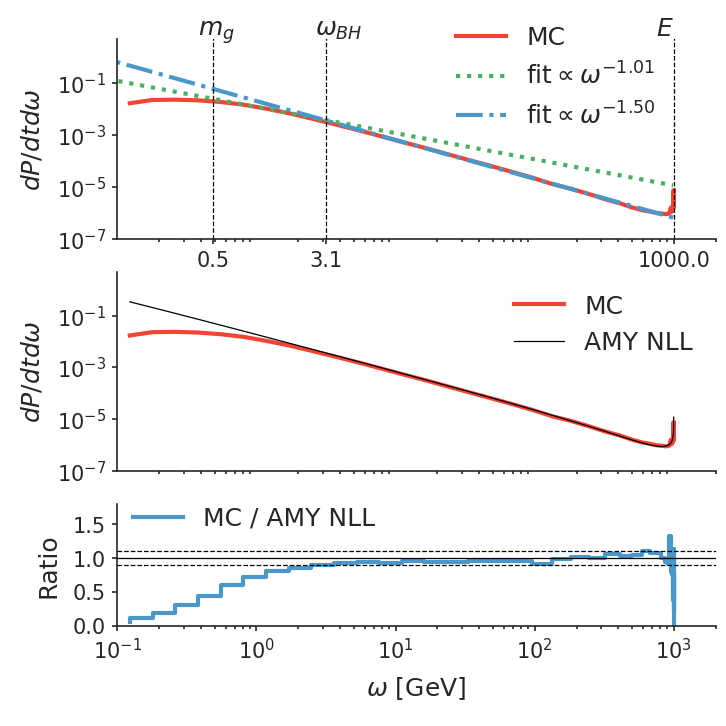
\includegraphics[width=\columnwidth]{spectrum.png}
\caption{Radiated gluon spectrum in an infinite medium from a quark of energy $E=1$ TeV, with a coupling constant $\alpha_s = 0.1$. The top frame shows the spectrum (red-dashed line) and power law fit (green-dotted and blue-dash-dotted lines) in different gluon energy ($0<\omega < E$) regions, separated by energy scales $m_\infty$, $\hat{q}_0\lambda_g^2 \sim 2\pi T$. The middle frame is the same calculation compared to the incoherent spectrum and the AMY semi-analytic result. The bottom frame is the ratio between the Monte-Carlo simulation and the semi-analytic calculation.}
\label{fig:spectrum}
\end{figure}

\begin{figure}
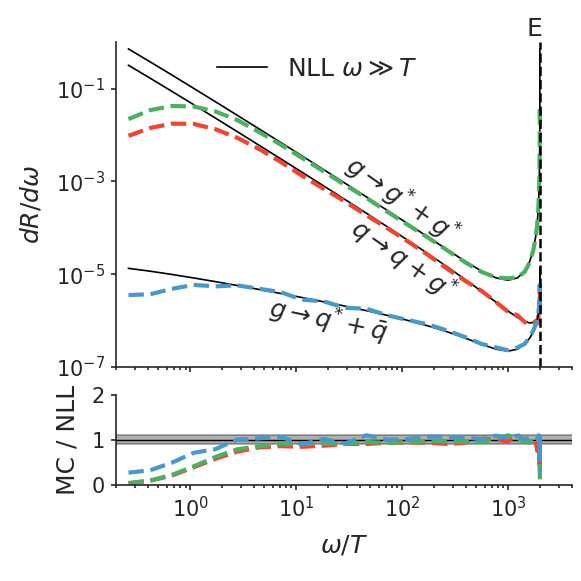
\includegraphics[width=\columnwidth]{channel_rate.png}
\caption{The splitting rate of $q\rightarrow q+g^*$, $g\rightarrow g+g^*$, and $g\rightarrow q^* + \bar{q}$ as a function of the parton energy labeled by the star. The mother parton with $E=1$ TeV evolves inside an infinite medium with $T=0.5$ GeV. The Monte Carlo results (thick dashed lines) are compared to the AMY NLL results (thin solid lines).}
\label{fig:channel_rate}
\end{figure}

\begin{figure}
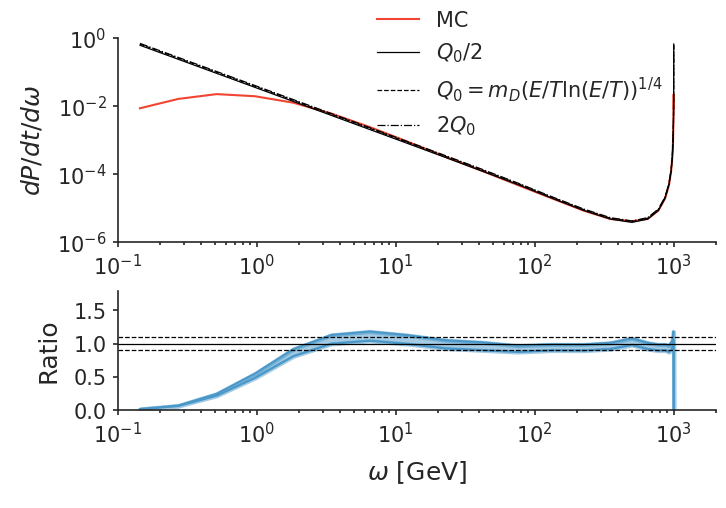
\includegraphics[width=\columnwidth]{running.png}
\caption{Comparison of modified Boltzmann simulation with AMY NLL calculation using running coupling of $\alpha_s$. The running scale in $\alpha_s(Q)$ is regulated at $\mu\pi T$ with $\mu=1,2$. The ratio between simulation and theory is shown in the bottom plot.}
\label{fig:running}
\end{figure}

In this section, we compare the splitting rate $dR/d\omega$ that comes out of the modified Boltzmann approach simulation to the NLL approximation in the infinite medium limit.

The differential rate in an infinite medium $dR/d\omega$ is shown in Figure \ref{fig:spectrum} for a 1 TeV quark splitting into a gluon and a quark.
The temperature of the medium is $T=0.5$ GeV, and a rather small coupling constant $\alpha_s = 0.1$.
Please also refer to Appendix \ref{app:tune-spectrum} for a full comparison varying both the parton energy and the coupling constant.
The horizontal axis is the radiated gluon energy.
In the upper plot, we divided the spectrum into different regions by the gluon thermal mass $m_\infty$ and an estimated Bethe-Heitler energy $\lambda_g m_D^2 \sim 2\pi T$.
The spectrum with above the is suppressed due the use of a finite mass.
In the Bethe-Heitler region $\omega < 2\pi T$, the spectrum scales like $\omega^{-1}$ which comes from the incoherent radiation rate.
In the LPM region $2\pi T < \omega < E$, the spectrum is dominated by coherent multiple scatterings and scales like $\omega^{-3/2}$.
The power-law fits in each domain are very close to the expected scaling.
In the middle plot, we compare the simulation to the AMY NLL approximation, with the ratio between the two shown in the bottom plot.
There is a good agreement in the LPM region between the simulation and the theory calculation, which we have used as guidance in developing our Monte-Carlo approach.

A comparison of the other channels $g\rightarrow g+g$ and $g\rightarrow q+\bar{q}$ to the theory calculations are shown in Figure \ref{fig:channel_rate}.
For the splitting parton energy much greater than temperature $\omega > 10 T$, the simulation agrees well with the theory. 

Finally, we compare the running coupling calculation with the theory curve in Fig. \ref{fig:running} for the $g\rightarrow g+g$ channel.
The theory curves (black lines) are obtained combining Eq. \ref{eq:AMY-LL} and Eq. \ref{eq:q3running}.
Different line styles correspond to the variation of the $Q_0$ value around its initial guess $m_D E/T \ln(E/T)$ by a factor of $2$ above and below.
For this 1 TeV parton, the scale $Q_0$ is actually very large and the running of $\alpha_s$ is rather slow, which explains the theory curve is not very sensitive to a factor of $4$ change in $Q_0$.
The simulation was performed using the running coupling prescription described in Section \ref{section:running}.
The overall shape of the spectrum in the deep LPM region is again well described by the modified Boltzmann simulation. 


\section{Towards phenomenological applications}\label{section:more}
In the previous section, we have shown that the modified Boltzmann equation simulation has a good agreement with the AMY NLL calculation for parton splitting in the LPM regime, for an infinite medium and fixed coupling case.
Towards future phenomenological application, we would like to investigate a few more complicated setup including a finite medium and an expanding medium.

\subsection{Results in a finite medium}
For calculation in a finite medium, there is an intricate interference pattern near the boundary which requires solving the original equation using a finite medium temperature profile. Or for the case of a thin medium, such effect can be analyzed order by order in the ``opacity ($L/\lambda$) expansion". 
One important outcome of a finite medium is the path-length dependent radiation rate for $L \lesssim \tau_f$, which is important for heavy-ion collisions phenomenology, considering the formation time of very energetic splitting can be comparable to the size of the QGP fireball.
Though the modified Boltzmann approach has been constructed to mimic the rate $dR/d\omega$ in the infinite medium limit, and does not recover the exact form of spectrum for a finite medium, it still predicts an $L$-dependent $dR/d\omega$ and we would like to check whether it is significantly different from the theory expectation.
The origination of the path-length dependence in the modified Boltzmann approach comes from that the gluon sampled at $t=t_0$ was not considered as independent object until $t = t_0+\tau_f$, meaning the splittings at time $t$ is initiated by inelastic processes at $t-\tau_f$.
As a result, in a semi-infinite medium with a step function like temperature profile, 
\begin{eqnarray}
T = \begin{cases}
0 , z<0\\
T_0, z>0
\end{cases}
\end{eqnarray}
there are no scattering centers at $L-\tau_f<0$ and thus introduces a $L$-dependent rate in this approach.

\begin{figure}
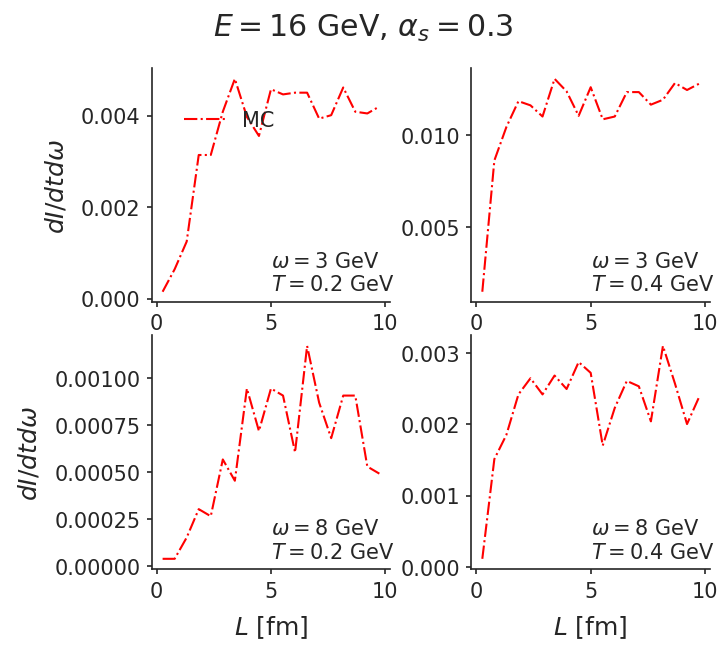
\includegraphics[width=\columnwidth]{spectrum_L.png}
\caption{Comparison of the path-length dependent energy-differential rate $dP/(dtd\omega)$ from the Monte-Carlo implementation using $\alpha_s = 0.3$ to the theoretical baseline calculation \cite{CaronHuot:2010bp}. The light quark energy is $16$ GeV.}
\label{fig:spectra-L-alphas=0.3}
\end{figure}

In Figure \ref{fig:spectra-L-alphas=0.3}, the $q\rightarrow q+g$ rate simulated in a semi-infinite medium is compared to the full calculations obtained from \cite{CaronHuot:2010bp}.
The energy of the quark is 16 GeV, and $\alpha_s = 0.3$.
The medium temperature of the left and the right columns are 0.2 GeV and 0.4 GeV respectively.
Top and bottom rows show the differential rates for the emitted gluon  energy $\omega = 3$ GeV and $\omega = 8$ GeV \footnote{In practical simulation, the rate are obtained by counting gluons within a finite energy range $\omega\pm 0.5$ GeV}.
The different rate $dR/d\omega$ are plotted as function of the path length $L$.
It is evident that theoretical rates (black solid lines) first grow approximately linearly with $L$ and then bend over to transit to $L$-independent ones.
The simulation describes the large $L$ limit well and also approximately captures the point at which the transition happens.
But there are systematic deviations compared to the theory calculations at small path-length.
Therefore it will be of great interest for future improvements to the current simulation approach at small path-length. 
For example, one possible solution would be using the results from the opacity expansion in the simulation for those splittings that happen close to the boundary and developing matching conditions to the approach we used for the deep LPM regime.

\subsection{Results in an expanding medium}
\begin{figure}
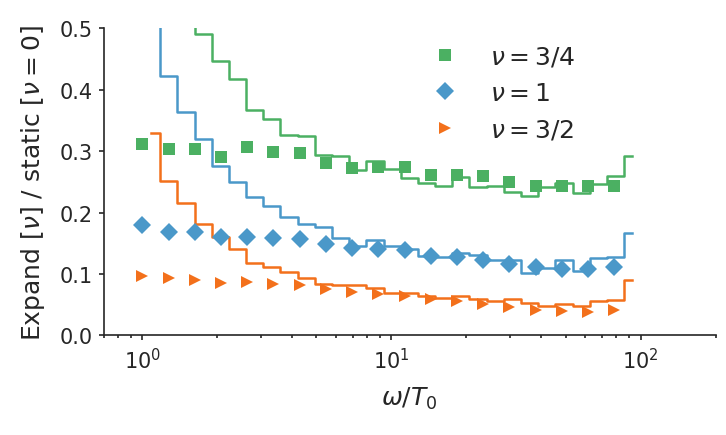
\includegraphics[width=\columnwidth]{spectrum_Bjorken.png}
\caption{The top frame shows the gluon radiation spectrum calculated with the the BDMPS formula (symbols) and Monte-Carlo simulations (lines) in a static medium ($\nu=1/2$), a slowly expanding medium ($\nu=5/7$) and a Bjorken expanding medium ($\nu\rightarrow 1$). In the bottom frame, we compute ratios of the analytic results and simulations between expanding cases and the static case. The parameters chosen are $\alpha_s=0.3$, $\tau_0 = 0.2$ fm/$c$, $L = 19.8$ fm/$c$, $T_0 = 1$ GeV.}
\label{fig:Bjorken-BDMPS}
\end{figure}

The expansion of the medium is another important feature of heavy-ion collision phenomenology.
The created QGP fireballs undergo dramatic expansion and causes the temperature of the medium at mid-rapidity to drop quickly in the first few fm$/c$.
This introduces another macroscopic scale in additional to the path length, which is the inverse medium expansion rate. 
In the context of this work, we shall define this expansion time scale as the inverse changing rate of $T^3$,
\begin{eqnarray}
\tau_{\textrm{ex}} = \left(\frac{d\ln(T^3)}{d \tau} \right)^{-1},
\end{eqnarray}
to be understood as the time scale over which the local $\hat{q}\propto T^3$ changes notably.
For simplicity, neglect the radial flow and parametrize the temperature profile as a power law fall-off function of the proper time at mid-rapidity,
\begin{eqnarray}
T(\tau; \nu)^3 = T_0^3\left(\frac{\tau_0}{\tau}\right)^{2-1/\nu},
\end{eqnarray}
where the static case is recovered when $\nu=1/2$, and $\nu=1$ corresponds to the temperature profile of a Bjorken flow.
The resultant expansion time is
\begin{eqnarray}
\tau_{\textrm{ex}} = \frac{\tau}{2-1/\nu}.
\end{eqnarray}
If this time scale is smaller than the formation time of the splitting, then the medium cannot be well approximated by having a constant temperature when we resumes the multiple scatterings.
Fortunately, in the current modified Boltzmann approach, since we propagate the splitting process in real time, the fast changing of the medium temperature does affect the multiple scatterings that contribute to this specific splitting.

Next we would like to compare the effect of expanding medium in the modified Boltzmann approach to the existing theoretical calculation.
The theoretical formula we used is obtained in the BDMPS framework 
by the authors of \cite{Baier:1998yf} using the power law type temperature profile,
\begin{eqnarray}
\frac{dP}{d\omega} &=& \frac{\alpha_s}{2\pi E}P_{q\rightarrow qg}(x)\mathfrak{Re}\int_{\tau_0}^{\tau_0+L}\frac{dt_f}{t_f}\int_{\tau_0}^{t_f}\frac{dt_i}{t_i} \frac{1}{\nu^2}\\
\nonumber
&& \left.\left[ I_{\nu-1}(z_i)K_{\nu-1}(z_f)-I_{\nu-1}(z_f)K_{\nu-1}(z_i)\right]^{-2}\right|_{\omega}^{\omega=\infty},\\
z_{i,f} &=& 2i\nu \sqrt{\frac{\hat{q}_g(1-x+C_F/C_A x^2)}{2(1-x)\omega}} \tau_0 \left( \frac{t_{i,f}}{\tau_0}\right) ^{1/2\nu}
\end{eqnarray}
for the $q\rightarrow q+g$ splitting.
For $\nu=1/2$, this expression reduces to the static BDMPS result \cite{Baier:1996kr}. 

As a remark, the BDMPS calculation considers the multiple-soft limit of the collision kernel and therefore does not include the logarithm that comes from the perturbative tail $1/q_\perp^4$. 
Accordingly, we turn off the large-$Q$ matrix-element scatterings and only retain diffusion plus diffusion-induced radiation components in our simulation.
Besides, $b=0.75$ is used without the logarithmic correction factor in Eq. \ref{eq:NLL-b}, and the same $\hat{q}_g = m_D^2 C_A\alpha_s T$ are input to the theory and the simulation.
To suppress other difference in the simulation and the theory, we will not make direct comparison of the spectrum $dP/d\omega$ to the BDMPS result, but instead comparing the ratio
\begin{eqnarray}
R_\nu = \frac{dP(T=T(\tau;\nu))/d\omega}{dP(T=T_0)/d\omega}
\end{eqnarray}
between the simulation and the theory to focus on the effect of a fast dropping temperature profile on the spectrum compared to the static case.

The medium expansion starts at $\tau_0=0.2$ fm/$c$ with $T_0=1$ GeV and stops at $\tau = 20$ fm/$c$.
We take four choices of the expansion rate $\nu = 1/2, 3/4, 1, 3/2$, corresponding to a static medium, a slowly expanding medium, Bjorken flow, and a faster-than-Bjorken expansion respectively.
The ratio $R_\nu$ from both theory and simulation are shown in Fig. \ref{fig:Bjorken-BDMPS} for a 100 GeV quark with $\alpha_s=0.3$.
In the deep-LPM region, the simulation describes the decreasing of medium-induced radiation due to the fast dropping of temperature.
In the future, we are looking forward to making direct comparison to the solution of Eq. \ref{eq:full-theory} with both varying temperature and radial flow effects.

\section{Summary and outlook}\label{section:summary}
We have investigated the modification to the incoherent Boltzmann transport approach to include the LPM effect for parton splitting processes in the deep LPM region, with the guidance from the next-to-leading-log solution of the AMY equation.
The running coupling effect has also implemented in this approach.
The overall level of agreement between the simulated results and theoretical calculations in the infinite medium limit is promising given the simplicity and limits of a Monte-Carlo procedure. 
Although it was developed for the deep LPM regime, the current approach captures qualitative features of the path-length dependence of medium induced splittings and the qualitative change of the spectrum shape in an expanding medium compared to the static case.
Of course, it is important to improve this method for the case of a thin medium.
Another primary interest would be a consistent inclusion of the heavy quark mass effect into the current approach.
We shall seek for improvements in these aspects in our future works.

Designing such a modified Boltzmann transport approach and comparing to theoretical calculations systematically has allowed us to reduce and estimate the uncertainty in implementing the medium induced splitting processes in the transport models. 
This is instrumental for performing an examination of theory assumptions and a more meaningful phenomenological extraction of jet transport properties in future model-to-data comparison.

\begin{acknowledgments}
SAB, WK and YX are supported by the U.S. Department of Energy Grant no. DE-FG02-05ER41367. WK is also supported by NSF grant OAC-1550225.
WK would like to thank Florian Senzel, Jean-Francois Paquet and Yacine Mehtar-Tani for helpful discussions.
\end{acknowledgments}

\begin{appendices}
\begin{figure}
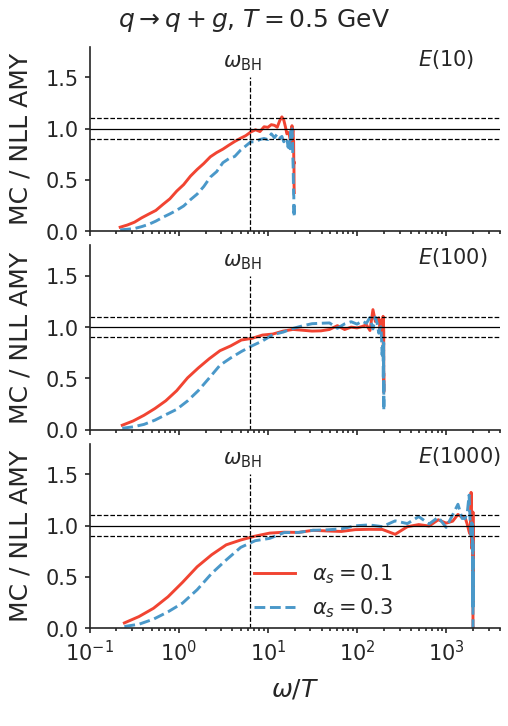
\includegraphics[width=\columnwidth]{spectrum_E_q2qg.png}
\caption{Ratios of Monte-Carlo calculated gluon emission spectra to the AMY NLL spectra (gray bands) and to the Gunion-Bertsch incoherent spectra (blue lines), using $\alpha_s = 0.1$. The quark energies are $E$ is 10, 50, 100, and 500 GeV as indicated by the rightmost vertical dashed lines in each subplot. The horizontal dashed lines denote $\pm 10\%$ deviation from unity.}
\label{fig:spectra-alphas=0.1}
\end{figure}

\begin{figure}
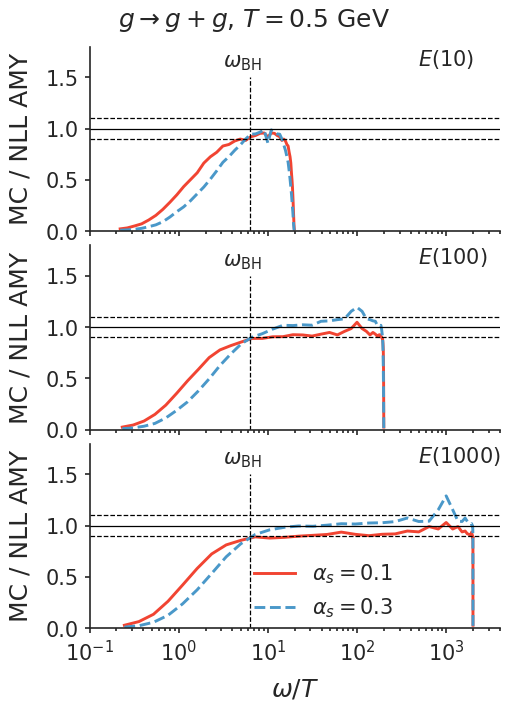
\includegraphics[width=\columnwidth]{spectrum_E_g2gg.png}
\caption{Ratios of Monte-Carlo calculated gluon emission spectra to the AMY NLL spectra (gray bands) and to the Gunion-Bertsch incoherent spectra (blue lines), using $\alpha_s = 0.1$. The quark energies are $E$ is 10, 50, 100, and 500 GeV as indicated by the rightmost vertical dashed lines in each subplot. The horizontal dashed lines denote $\pm 10\%$ deviation from unity.}
\label{fig:spectra-alphas=0.1}
\end{figure}

\begin{figure}
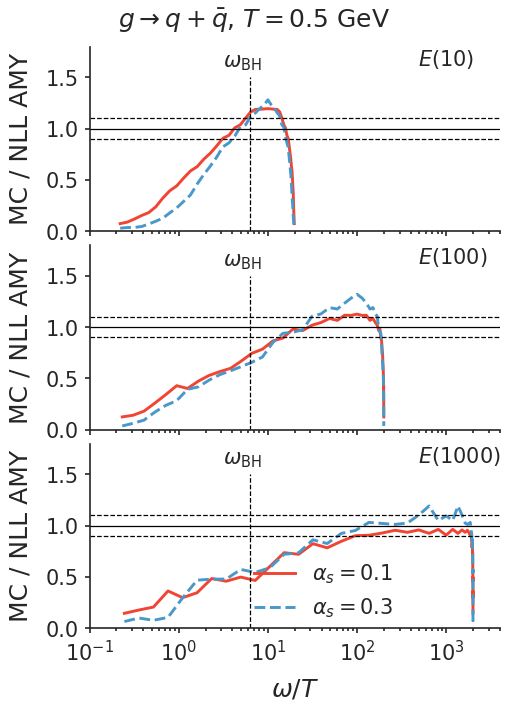
\includegraphics[width=\columnwidth]{spectrum_E_g2qqbar.png}
\caption{Ratios of Monte-Carlo calculated gluon emission spectra to the AMY NLL spectra (gray bands) and to the Gunion-Bertsch incoherent spectra (blue lines), using $\alpha_s = 0.1$. The quark energies are $E$ is 10, 50, 100, and 500 GeV as indicated by the rightmost vertical dashed lines in each subplot. The horizontal dashed lines denote $\pm 10\%$ deviation from unity.}
\label{fig:spectra-alphas=0.1}
\end{figure}

\section{Energy and coupling constant dependence of the splitting rate}\label{app:tune-spectrum}
It is important to be aware of the known discrepancies between the Monte-Carlo implementation and the theory baseline, particularly if one investigates an observable that is sensitive to the details of the radiation spectra. 
In this appendix, we provide comparisons of radiation spectra at different values of energy and coupling constant for the reader's references.
Figure \ref{fig:spectra-alphas=0.1} and Figure \ref{fig:spectra-alphas=0.3} shows calculation using $\alpha_s = 0.1$ and $0.3$.
Within in each figure, different subplots vary the quark energy.
The gray bands are the ratios between the simulations and the AMY-NLL results (plotted for $\pi T < \omega < E$) and the blue lines are the ratios between the full simulations and the incoherent simulations (the Gunion-Bertsch rate, plotted for $0.1$ GeV $< \omega < 4\pi T $).
We notice that there are residual systematic discrepancies, but the overall difference is controlled within $\pm 15\%$ for the coupling constants, temperatures and energies under consideration.

\section{The $2\rightarrow 3$ matrix-elements}

\end{appendices}
\bibliography{mclpm} 
\end{document}
